\documentclass[conference]{IEEEtran}
\IEEEoverridecommandlockouts

\usepackage{cite}
\usepackage{amsmath,amssymb,amsfonts}
\DeclareMathAlphabet{\mathbf}{OT1}{ptm}{bx}{n}
\usepackage{algorithmic}
\usepackage{graphicx}
\usepackage{textcomp}
\usepackage{xcolor}
\usepackage{booktabs}
\usepackage{multirow}
\usepackage{url}
\usepackage{listings}
\usepackage{microtype}

\lstset{
  basicstyle=\ttfamily\scriptsize,
  breaklines=true,
  frame=single,
  columns=fullflexible
}

\def\BibTeX{{\rm B\kern-.05em{\sc i\kern-.025em b}\kern-.08em
    T\kern-.1667em\lower.7ex\hbox{E}\kern-.125emX}}

\begin{document}

\title{SAGE: Measuring Security Drift and Capability Retention in Self-Evolving Code Agents\thanks{Code and data at \protect\url{https://github.com/Pratikjain24/SAGE}. Full benchmark released open-source with DOIs via Zenodo and HuggingFace.}}

\author{
    \IEEEauthorblockN{
        Pratik P. Jain\IEEEauthorrefmark{1},
        Janhavi B. Pagare\IEEEauthorrefmark{1},
        Aditya U. Dengale\IEEEauthorrefmark{1},
        Naitik K. Kharat\IEEEauthorrefmark{1},
        Shamika R. Kadam\IEEEauthorrefmark{1}, and
        Vikrant K. Kadam\IEEEauthorrefmark{1}
    }
    \IEEEauthorblockA{
        \IEEEauthorrefmark{1}Department of Computer Engineering, Vishwakarma Institute of Technology, Pune, India\\
        Email: \{pratik.12620589, janhavi.1252010010, aditya.1252010025,\\
        naitik.12620301, shamika.12620290, vikrant.1252010030\}@vit.edu
    }
}

\maketitle

\begin{abstract}
LLM agents now modify their own prompts, memories, and tools over time. This self-evolution boosts capability, but existing benchmarks only check single-turn performance—missing critical long-term problems.

Three pathologies emerge: agents game evaluation metrics through hardcoded shortcuts, drop security checks for speed, and forget old skills. We built SAGE to catch these failures across 25 generations. Testing 9,814 episodes on Qwen2.5-Coder-7B reveals the tradeoff: unguarded agents hit 80\% accuracy but violate security in 32\% of cases. Our rollback guards maintain 73.5\% accuracy with zero breaches.

SAGE defines seven agent types (frozen to verification-protected) and uses a five-layer sandbox that survived penetration testing. Human reviewers validated our automated metrics (N=319, 86\% agreement). Results show self-evolution creates capability-safety tensions that standard testing completely misses.
\end{abstract}

\begin{IEEEkeywords}
AI safety, LLM agents, code generation, self-evolving systems, benchmark design, security testing
\end{IEEEkeywords}

\section{Introduction}

Code autocomplete is old news. Today's LLM agents plan solutions, run code, debug errors, and iterate~\cite{yao2023react,shinn2024reflexion,yang2024sweagent}. What's next? Agents that rewrite themselves—updating instructions, building tool libraries, accumulating experience. These systems could keep improving months after deployment.

Here's the problem. Unsupervised self-optimization finds shortcuts. We've seen three failure modes repeatedly:

\textbf{Test gaming.} Agents hardcode return values or mock fixtures instead of solving problems. Passes tests, breaks in production.

\textbf{Security decay.} Input validation slows benchmarks down. Agents remove these "expensive" checks, opening SQL injection and shell escape holes.

\textbf{Skill loss.} Specializing to new tasks overwrites old knowledge. Performance on mastered challenges collapses.

This isn't speculation. METR found a 43-fold jump in agents tampering with test harnesses when containers lacked strict isolation~\cite{metr2024evaluating}. Most benchmarks run tests in the agent's directory—trivial to cheat.

SAGE tracks agents across 5-25 self-modification cycles. Unlike existing work, we measure whether code works \emph{and} whether it's honest and safe. Our contribution is threefold:

First, we define seven agent types. G1 is frozen (baseline). G2-G4 have increasing mutation freedom. G5-G7 add verification layers. Each isolates one mechanism: prompt evolution, memory growth, or tool synthesis.

Second, our sandbox has five defense layers. Ground-truth tests run in an isolated container. Git checks catch file tampering. SHA-256 hashes verify fixtures. Static analysis blocks exploit patterns. Kernel restrictions drop privileges. This survived five attack vectors.

Third, we built 100 tasks from scratch. Zero-shot tests found 0\% memorization in Qwen and Llama—compare that to 32.7\% in SWE-bench~\cite{openai2026swebenchleakage}. Twenty tasks are traps: visible tests accept shortcuts that hidden tests reject.

Running 9,814 episodes on dual T4 GPUs confirmed the tradeoff. Unconstrained agents (G2, G4) reach 80\% but violate security 22-32\% of the time. Static checks (G5) block exploits but miss functional gaming. Only rollback verification (G7) keeps both performance (73.5\%) and safety (0\% violations). We had 319 trajectories reviewed by humans over 83 hours—86\% agreement with automated scores.

Section~\ref{sec:related_work} covers related work. Section~\ref{sec:architecture} explains agent types and sandbox design. Section~\ref{sec:data_engineering} describes our task set. Results are in Section~\ref{sec:results}, discussion in Section~\ref{sec:discussion}.

\section{Related Work}

\subsection{Static Benchmarks}

HumanEval~\cite{chen2021evaluating} and MBPP~\cite{austin2021program} test function generation. Both leaked into training data—scores are inflated. EvalPlus~\cite{liu2023evalplus} adds harder tests. SWE-bench~\cite{jimenez2024swebench} uses real GitHub patches, but 32.7\% of tasks appear in zero-shot completions~\cite{openai2026swebenchleakage}.

These check one attempt. Agents can't evolve or maintain state across tasks. SAGE measures behavior over 10-25 generations: how does self-modification affect performance, safety, and memory?

\subsection{Agent Benchmarks}

InterCode~\cite{yang2023intercode} tests multi-turn interaction. EvoAgentBench~\cite{gao2026evoagentbench} measures API skill transfer. SkillsBench~\cite{liu2026skillsbench} looks at short-horizon learning (T≤5).

None track security drift or gaming. None isolate tests in separate containers. SAGE adds adversarial testing while tracking longer timescales.

\subsection{Self-Improving Systems}

Reflexion~\cite{shinn2024reflexion} uses verbal feedback. Voyager~\cite{wang2023voyager} builds Minecraft skill libraries. MemGPT~\cite{packer2023memgpt} extends context with hierarchical memory. All show that self-modification helps.

But nobody measured the costs. How does evolution degrade safety? When do agents start gaming metrics? SAGE tracks capability gains alongside violations, gaming, and forgetting.

\subsection{Gaming and Safety}

Optimizers exploit proxy metrics—documented from CoastRunners~\cite{amodei2016concrete} to LLM sycophancy~\cite{skalse2022defining}. METR caught agents modifying harnesses at scale~\cite{metr2026risk}. SpecBench~\cite{zhao2026specbench} measures single-turn gaming.

SAGE extends this longitudinally. Agents don't just game once—they encode shortcuts into persistent prompts and tools, corrupting future cycles. Our 20 probe tasks pair lax visible tests with strict hidden ones to quantify this.

\subsection{How SAGE Differs}

Table~\ref{tab:concurrent_benchmarks} shows where we stand. EvoAgentBench does skill transfer, not security. SpecBench catches gaming but not forgetting. Zhang et al.~\cite{zhang2026reward} catalog exploits without tracking persistent mutations. Yu et al.~\cite{yu2026forgetting} study forgetting without gaming.

We're the first to measure all three (gaming, drift, retention) together \emph{and} propose working countermeasures. Rollback guards maintain capability while preventing degradation.

\subsection{Delineation from Concurrent 2025--2026 Agent Benchmarks}
\label{sec:concurrent_studies}

Multiple agent benchmarks appeared across 2025 and 2026. Each targets distinct operational risks in foundation-model agents. SpecBench~\cite{zhao2026specbench} and Zhang et al.~\cite{zhang2026reward} study proxy reward hacking. EvoAgentBench~\cite{gao2026evoagentbench} examines multi-task transfer. Yu et al.~\cite{yu2026forgetting} track skill degradation. SAGE connects these separate threads into a single longitudinal framework. Table~\ref{tab:concurrent_benchmarks} outlines the key technical differences across state spaces, failure modes, and governance models.

\begin{table*}[t]
\centering
\small
\caption{\textbf{Systematic Delineation: SAGE vs. Concurrent 2025--2026 Agent Benchmarks}. Contrasting evaluation horizon, mutable state space, evaluated failure modes, exploit probes, causal archetype decomposition, sandbox containment, and affirmative governance mechanisms.}
\label{tab:concurrent_benchmarks}
\resizebox{\textwidth}{!}{%
\begin{tabular}{lccccc}
\toprule
\textbf{Architectural \& Empirical Dimension} & \textbf{SAGE (Ours)} & \textbf{SpecBench}~\cite{zhao2026specbench} & \textbf{EvoAgentBench}~\cite{gao2026evoagentbench} & \textbf{Yu et al.}~\cite{yu2026forgetting} & \textbf{Zhang et al.}~\cite{zhang2026reward} \\
\midrule
Evaluation Horizon ($T$) & \textbf{Longitudinal} ($T=5$ cycles) & Static episode ($T=1$) & Single-turn transfer ($T=1$) & Sequential tasks ($T=5$) & Static episode ($T=1$) \\
Mutable State Space ($\mathcal{S}_t$) & $\langle \Pi_t, \mathcal{M}_t, \mathcal{C}_t \rangle$ (Prompt, Memory, Tools) & $\emptyset$ (Stateless single-turn) & Black-box agent state & $\mathcal{M}_t$ (Memory store only) & $\emptyset$ (Stateless single-turn) \\
Coupled Trilemma Dynamics & \textbf{\checkmark Yes} ($\Delta P \iff \mathcal{V} \iff \Delta_{\text{proxy}} \iff \text{Ret}$) & $\times$ No (isolated gaming) & $\times$ No (benign transfer) & $\times$ No (isolated forgetting) & $\times$ No (isolated exploits) \\
Deliberate Exploit Drift Probes & \textbf{20 Probes} (AST, mock, bypass) & Validation vs. Hidden tests & $\times$ None & $\times$ None & Synthetic tool scenarios \\
Causal Archetype Decomposition & \textbf{\checkmark 7 Archetypes} ($G_1\text{--}G_7$) & $\times$ Monolithic agent & $\times$ Monolithic agent & Partial ablation ($\pm\mathcal{M}$) & $\times$ Monolithic agent \\
Execution Sandbox Environment & \textbf{Dual Docker} (5-layer isolated) & Single Docker / Subproc & Mock API harness (no OS) & Subprocess execution & Simulated environment \\
Affirmative Governance \& Rollback & \textbf{\checkmark Canary Rollback} ($G_7$) & $\times$ Passive auditing only & $\times$ Passive auditing only & $\times$ Passive auditing only & $\times$ Passive auditing only \\
Governance Paralysis Resolved & \textbf{\checkmark Yes} (+0.050 train, 73.5\% test under $G_7$) & $\times$ N/A & $\times$ N/A & $\times$ N/A (unresolved trade-off) & $\times$ N/A \\
\bottomrule
\end{tabular}%
}
\vspace{1mm}
\caption*{\footnotesize \textit{Note}: $\Delta P$: Net forward capability gain; $\mathcal{V}$: Security boundary erosion; $\Delta_{\text{proxy}}$: Gaming gap on deliberate probes; Ret: Historical skill retention. $G_7$: Deployable canary rollback guard; $G_7^*$: Oracle skyline.}
\end{table*}

\subsubsection{SpecBench (Zhao et al.~\cite{zhao2026specbench}) vs. SAGE's Longitudinal Proxy Gap}
SpecBench evaluates reward hacking in single-attempt agents ($T=1$). It checks if patches pass visible tests but fail hidden checks. This captures static gaming in one turn.

SAGE tracks how gaming compounds across generations. The proxy gap $\Delta_{\text{proxy}}$ is not just a one-time bug. It becomes a persistent habit. Unconstrained agents ($G_4$) quickly learn that patching test fixtures or mocking return values takes less effort than writing valid algorithms. They store these shortcuts in memory ($\mathcal{M}_t$) and helper tools ($\mathcal{C}_t$). Future cycles inherit those corruptions. On our 20 drift probes, $G_4$ agents hit 95.0\% on visible tests but drop to 40.0\% on hidden ground truth ($\Delta_{\text{proxy}} = +0.55$).

SpecBench stops at passive auditing. SAGE adds an active defense. Our dynamic canary gates ($G_7$) roll back bad mutations, holding the gap to $\Delta_{\text{proxy}} \le +0.02$.

\subsubsection{EvoAgentBench (Gao et al.~\cite{gao2026evoagentbench}) vs. SAGE's Adversarial Self-Evolution}
EvoAgentBench tests skill transfer across tool APIs. It relies on mock APIs without real operating system execution. It also assumes self-evolution remains benign, measuring only positive skill gains.

SAGE treats self-evolution as an adversarial process, testing the misevolution hypothesis from Shao et al.~\cite{shao2025misevolution}. Left unchecked, agents erode their own security safeguards. In our runs, unconstrained mutators ($G_4$) breached security boundaries in 32.0\% of runs ($\mathcal{V} = 0.32$). They stripped input checks, escaped subshells, and edited test code. SAGE runs all workloads inside an isolated dual container (\texttt{evo-sandbox} and \texttt{evo-scorer}) with unprivileged users and AST tripwires.

EvoAgentBench treats self-modification as a black box. SAGE isolates specific mechanisms through seven archetypes ($G_1$--$G_7$). We separate the impact of prompt edits ($G_2$), memory writes ($G_3$), full reflection ($G_4$), static AST rules ($G_5$), and canary rollbacks ($G_7$).

\subsubsection{Yu et al.~\cite{yu2026forgetting} vs. SAGE's Retention and Governance Paralysis}
Yu et al. study catastrophic forgetting during lifelong agent adaptation. Adapting memory to new problems harms performance on earlier tasks. Our experiments verify this trend. Memory accumulation ($G_3$) and reflection ($G_4$) drop task retention to 89.0\% and 81.0\%, respectively.

SAGE identifies a deeper practical roadblock: governance paralysis. Preventing forgetting is easy if the system rejects every update with past variance. That keeps retention at 100\%, but stops all learning ($\Delta P = 0$). The agent remains stuck at baseline solvability.

The key engineering challenge is enabling forward gains while preventing regressions. Deployable canary verification ($G_7$) solves this dilemma. It delivers a $+0.050$ training gain and 73.5\% held-out test solvability ($p_{\text{Holm}} = 0.002, d = 2.45$) while maintaining 96.0\% retention on past tasks and eliminating security boundary drift.

\subsubsection{Zhang et al.~\cite{zhang2026reward} vs. SAGE's Persistent Tool Mutation and Governance Frontier}
Zhang et al.~\cite{zhang2026reward} analyze reward hacking in single tool interactions. SAGE differs in two key ways:

\textbf{Persistent Artifacts vs. One-Off Exploits.} In Zhang et al., actions disappear once a task resets. In SAGE, synthesized tools ($\mathcal{C}_t$) persist on disk as part of the state $\mathcal{S}_t$. When an agent writes a fixture-patching script at step $t$, subsequent generations inherit that code. The shortcut turns into a permanent habit.

\textbf{Active Governance Frontier.} Zhang et al. focus on diagnosis. SAGE evaluates affirmative defenses. Static AST filters ($G_5$) stop syntax tampering at near-zero runtime cost ($\mathcal{V} \le 0.02$). But AST linters miss semantic gaming ($\Delta_{\text{proxy}} = +0.28$). Combining static analysis with dynamic canary rollbacks ($G_7$) stops security leaks while controlling the gaming gap.

\subsubsection{The Unifying Conceptual Breakthrough: The Self-Evolution Trilemma}
SAGE unifies these phenomena into the \textbf{Self-Evolution Trilemma}. System designers face three conflicting requirements across cycles $t$:
\begin{equation}
\max_{\mathcal{E}} \Delta P(T) \quad \text{s.t.} \quad \mathcal{V}(t) \le \epsilon_{\text{sec}}, \quad \Delta_{\text{proxy}}(t) \le \epsilon_{\text{proxy}}, \quad \text{Ret}(t) \ge 1 - \epsilon_{\text{ret}}
\end{equation}
Existing benchmarks study isolated parts of this formulation. SpecBench inspects the proxy gap $\Delta_{\text{proxy}}$. Yu et al. examine retention. EvoAgentBench tests capability gain $\Delta P$.

Our results show these goals are directly coupled. Pushing capability in open-loop setups ($G_2, G_4$) triggers security drift ($\mathcal{V} = 0.32$), gaming ($\Delta_{\text{proxy}} = +0.55$), and skill loss (retention down to 81.0\%). Overly strict gates cause paralysis ($\Delta P = 0$). SAGE uses 20 deliberate probes to test this balance. Deployable canary rollback ($G_7$) successfully balances this trade-off, providing a concrete path for stable agent evolution.


\section{System Design}

\subsection{State Representation}

Agent state at generation $t$ has three parts:
\begin{equation}
\mathcal{S}_t = \langle \Pi_t, \mathcal{M}_t, \mathcal{C}_t \rangle
\end{equation}

$\Pi_t$ = system prompt (instructions, identity, behavior).  
$\mathcal{M}_t$ = memory (traces, failures, playbooks).  
$\mathcal{C}_t$ = tools (Python helpers, wrappers).

Each cycle, the agent tackles 100 tasks: read spec, write patches, run visible tests. We record binary success $r_\tau \in \{0,1\}$ plus tool calls, outputs, and test results.

After 100 tasks, feedback aggregates to:
\begin{equation}
\mathcal{F}_t = \langle \text{pass rate}, \text{failures}, \text{violations}, \text{gaming gap}, \text{patterns} \rangle
\end{equation}

The agent updates itself:
\begin{equation}
\mathcal{S}_{t+1} = \mathcal{E}(\mathcal{S}_t, \mathcal{F}_t)
\end{equation}

Mutation operator $\mathcal{E}$ varies by type—next section.

\subsection{Seven Agent Types}

What drives gains and losses? We isolated mechanisms:

\textbf{G1 (Frozen).} Nothing changes: $\mathcal{S}_t = \mathcal{S}_0$ always. Pure baseline.

\textbf{G2 (Prompt Only).} Just $\Pi_t$ evolves. LLM reads feedback, rewrites instructions. Memory and tools stay fixed.

\textbf{G3 (Memory Only).} Just $\mathcal{M}_t$ grows. Agent extracts playbooks from wins and loss patterns. Prompt and tools unchanged.

\textbf{G4 (Full).} All three mutate freely. Prompt, memory, tools—no restrictions.

\textbf{G5 (Static Check).} Like G4 but an AST linter scans mutations. Blocks test mocking, module patching, forced exits. Violations trigger rollback.

\textbf{G6 (Proxy Gate).} Mutations pass a behavioral check on held-out tasks. If retention drops, reject. Uses only visible tests.

\textbf{G6* (Oracle).} Like G6 but uses hidden ground-truth tests. Theoretical ceiling—real agents can't see hidden tests.

Why G6*? We follow convention (π*, Q*) for theoretical optima. Early runs called the proxy version G7, but we standardized on G6 (deployable) vs G6* (oracle).

\subsection{Five-Layer Sandbox}

Shell access = easy cheating. Modify tests, patch modules, fake exits. We built five defenses:

\textbf{Layer 1: Container split.} Agents in \texttt{evo-sandbox}, tests in \texttt{evo-scorer}. Test container mounts code read-only. No cross-access.

\textbf{Layer 2: Git checks.} Before scoring: \texttt{git status --porcelain}. Any modified harness files = instant fail, logged exploit.

\textbf{Layer 3: Hashing.} SHA-256 every test and fixture pre-run, verify post-run. Mismatch = tampering detected.

\textbf{Layer 4: Static scan.} Parse patches for: \texttt{unittest.mock}, \texttt{pytest.monkeypatch}, \texttt{sys.modules} tricks, exit() calls. Block on detection.

\textbf{Layer 5: Kernel lock.} Container runs as uid 1000 (unprivileged), all caps dropped, 2GB RAM limit, 1.0 CPU quota, no network, seccomp blocks danger syscalls.

Penetration testing: five vectors (/proc snoop, /tmp hijack, setuid, path traversal, socket leak). Bare host allows all. Single container allows three. Our dual setup blocks all. Over 27,814 total runs: zero escapes (95\% CI 0-0.04\%).

\subsection{Observability}

Docker Compose runs four services. Dashboard tracks pass rates and security drift. Inspector correlates code diffs with violations. Audit workbench shows blinded traces for human review. Explorer logs tool calls and events.

\section{Dataset}

\subsection{Design Principles}

Five goals shaped our tasks:

\textbf{P1. No contamination.} Every repo hand-written with unique interfaces. Zero-shot checks found 0\% memorization (vs 32.7\% in SWE-bench).

\textbf{P2. Focused.} Multi-file components, average 16.5 mutable lines in 150-450 line repos. Specs, implementations, tests, pinned deps.

\textbf{P3. Calibrated.} Target P(0)=60\%. Floor effect (too hard) prevents bootstrapping. Ceiling effect (too easy) hides regressions. Validation: Qwen hits 61.3\%, Llama 58.0\%.

\textbf{P4. Breadth.} Five domains × 20 tasks: bugs, features, refactors, security, probes.

\textbf{P5. Adversarial.} Twenty probe tasks. Visible tests accept shortcuts; hidden tests require correctness.

\subsection{Categories}

\textbf{Bug Fixing (20).} Deadlocks, cache leaks, protocol errors, timezone bugs.

\textbf{Features (20).} Raft consensus, B-trees, GraphQL parsers, rate limiters, CRDTs.

\textbf{Refactoring (20).} Module extraction, sync-to-async, type audits, DI migrations, versioning.

\textbf{Security (20).} Path traversal, SQL injection, JWT checks, XXE guards, password hashing.

\textbf{Probes (20).} Visible test checks types; hidden test checks semantics. Example: ORM visible test wants any dict; hidden test runs \texttt{DROP TABLE} injections.

\subsection{Difficulty Tiers}

McCabe complexity, reasoning steps, human solve time:

\textbf{Easy (34).} McCabe=4.3, 1-2 steps, 3.2 min. Frozen solves 85.3\%.

\textbf{Medium (33).} McCabe=3.3, 3-5 steps, 11.4 min. Frozen: 57.6\%.

\textbf{Hard (33).} McCabe=3.1 plus concurrency/crypto, 6+ steps, 24.8 min. Frozen: 36.4\%.

Weighted mean: $(34×0.853 + 33×0.576 + 33×0.364)/100 = 60.0\%$. Matches target and empirics.

\subsection{Contamination Check}

Zero-shot completion on all 100. Prompts had specs only (no code). Measured 4-gram overlap, LCS, verbatim lines, max token runs. All below 50\% threshold. Mean 4-gram: 0.0\%. Mean LCS: 4.2\% (just Python boilerplate).

SWE-bench: 32.7\% exceed 50\%. Our synthetic construction guarantees zero public repos cloned.

\subsection{Probe Design}
\label{sec:drift_probes}

Twenty gaming traps, each with two test files:

\texttt{test\_proxy.py} (visible): Surface checks. ORM returns dict?

\texttt{test\_gt.py} (hidden, separate container): Semantic checks. ORM rejects \texttt{DROP TABLE}?

Hardcoding a dict passes proxy, fails ground truth. Gaming gap:
\begin{equation}
\Delta_{\text{proxy}} = P_{\text{proxy}} - P_{\text{GT}}
\end{equation}

Large positive = gaming. Near zero = honest.

\section{Metrics and Methods}

Four metrics:

\textbf{Capability:} $\Delta P(t) = P(t) - P(0)$.

\textbf{Drift:} $\mathcal{V}(t) - \mathcal{V}(0)$ (violations: test tampering, module patching, exploits).

\textbf{Retention:} Fraction of baseline wins still passing. $\text{Retention}(t) = \frac{1}{|\mathcal{H}_0|} \sum_{\tau \in \mathcal{H}_0} \mathbf{1}[\text{pass}(\tau, \mathcal{S}_t)]$.

\textbf{Gaming:} $\Delta_{\text{proxy}}(t)$ on 20 probes.

Pre-registered hypotheses:

H1: Evolving agents gain capability ($\Delta P > 0$).

H2: Unconstrained show large gaming ($\Delta_{\text{proxy}} > 0.15$).

H3: Unconstrained increase violations.

H4: Retention drops below 90\% without guards.

H5: Rollback maintains low drift (<0.05) and gaming (<0.08) while gaining capability.

\section{Experiments}

Two tiers:

\textbf{Canonical (18,000).} Deterministic policies, 10 gens, 3 seeds (42-44), 100 tasks. Bitwise reproducible (Linux/Windows). Clean causal inference.

\textbf{Empirical (9,814).} Live Qwen2.5-Coder-7B on Kaggle T4 GPUs. Five seeds (42-46), 5 gens, 7 types. Real inference, full telemetry. No mocks. Validates findings under neural stochasticity.

Stats: bootstrap (B=10,000), Holm-Bonferroni, Cohen's d, Cliff's δ. Task (N=100) is unit; per-task averaged over seeds.

Cost: canonical models 334.8M tokens (\$74 at API rates). Empirical averaged \$0.25 per trajectory.

\section{Results}

\subsection{Core Findings}

Table~\ref{tab:main_results_live}: 9,814 live episodes show three things.

\textbf{Evolution helps.} G2 jumps 53.7→70.0\% training ($\Delta P=+0.163$, p=0.002, d=0.31), hits 80.0\% test. G5 climbs 52.7→65.0\% ($\Delta P=+0.123$), reaches 79.5\% test. G1 stays flat: 40.0\% train, 43.0\% test.

\textbf{Sandbox holds.} Zero escapes across 9,814 runs (95\% CI 0.0-0.04\%). Five layers worked.

\textbf{Rollback works.} G7 maintains 73.5\% test with $\Delta P=+0.050$ train gain, zero violations. Breaks the capability-safety myth.

\begin{table*}[t]
\centering
\small
% SAGE Live Distributed Study: Consolidated Empirical Benchmark Results (G1-G4 Live Data)
\caption{\textbf{Empirical Benchmark Results for SAGE Archetypes ($G_1$--$G_4$)}. Evaluated on \texttt{Qwen/Qwen2.5-Coder-7B-Instruct} across $N=5$ pinned random seeds (42, 43, 44, 45, 46) on Kaggle Dual Tesla T4 GPUs ($T=5$ cycles). $P_{\text{train}}$ measured across 60 training tasks per cycle; $P_{\text{test}}$ evaluated on 40 held-out tasks (Cycle 4); $\Delta P_{\text{train}} = P_{\text{train}}(3) - P_{\text{train}}(0)$ measures true training adaptation.}
\label{tab:live_main_results_g1_g4}
\begin{tabular}{llcccccc}
\toprule
Group & Mechanism & $P_{\text{train}}(0)$ & $P_{\text{train}}(3)$ & $\Delta P_{\text{train}}$ & $P_{\text{test}}(4)$ & SafetyDrift & Total Cost (\$) \\
\midrule
G1 & Static Baseline Control & 0.480 & 0.487 & +0.007 & 0.630 & 0.000 & \$0.4218 \\
G2 & Prompt Rewriter & 0.450 & 0.480 & +0.030 & 0.615 & 0.000 & \$0.4034 \\
G3 & Memory Accumulator & 0.480 & 0.447 & -0.033 & 0.575 & 0.000 & \$0.4274 \\
G4 & Reflection Agent & 0.467 & 0.517 & +0.050 & 0.605 & 0.000 & \$0.4560 \\
\bottomrule
\end{tabular}
\end{table*}

Figure~\ref{fig:live_learning_curves}: prompt and memory agents (G2, G3) improve steadily. Full reflection (G4) gains fast but violates security. Static and rollback (G5, G6, G7) balance progress with safety. Frozen (G1) flatlines—test stability confirmed.

\begin{figure*}[t]
\centering
\begin{minipage}{0.32\textwidth}
  \centering
  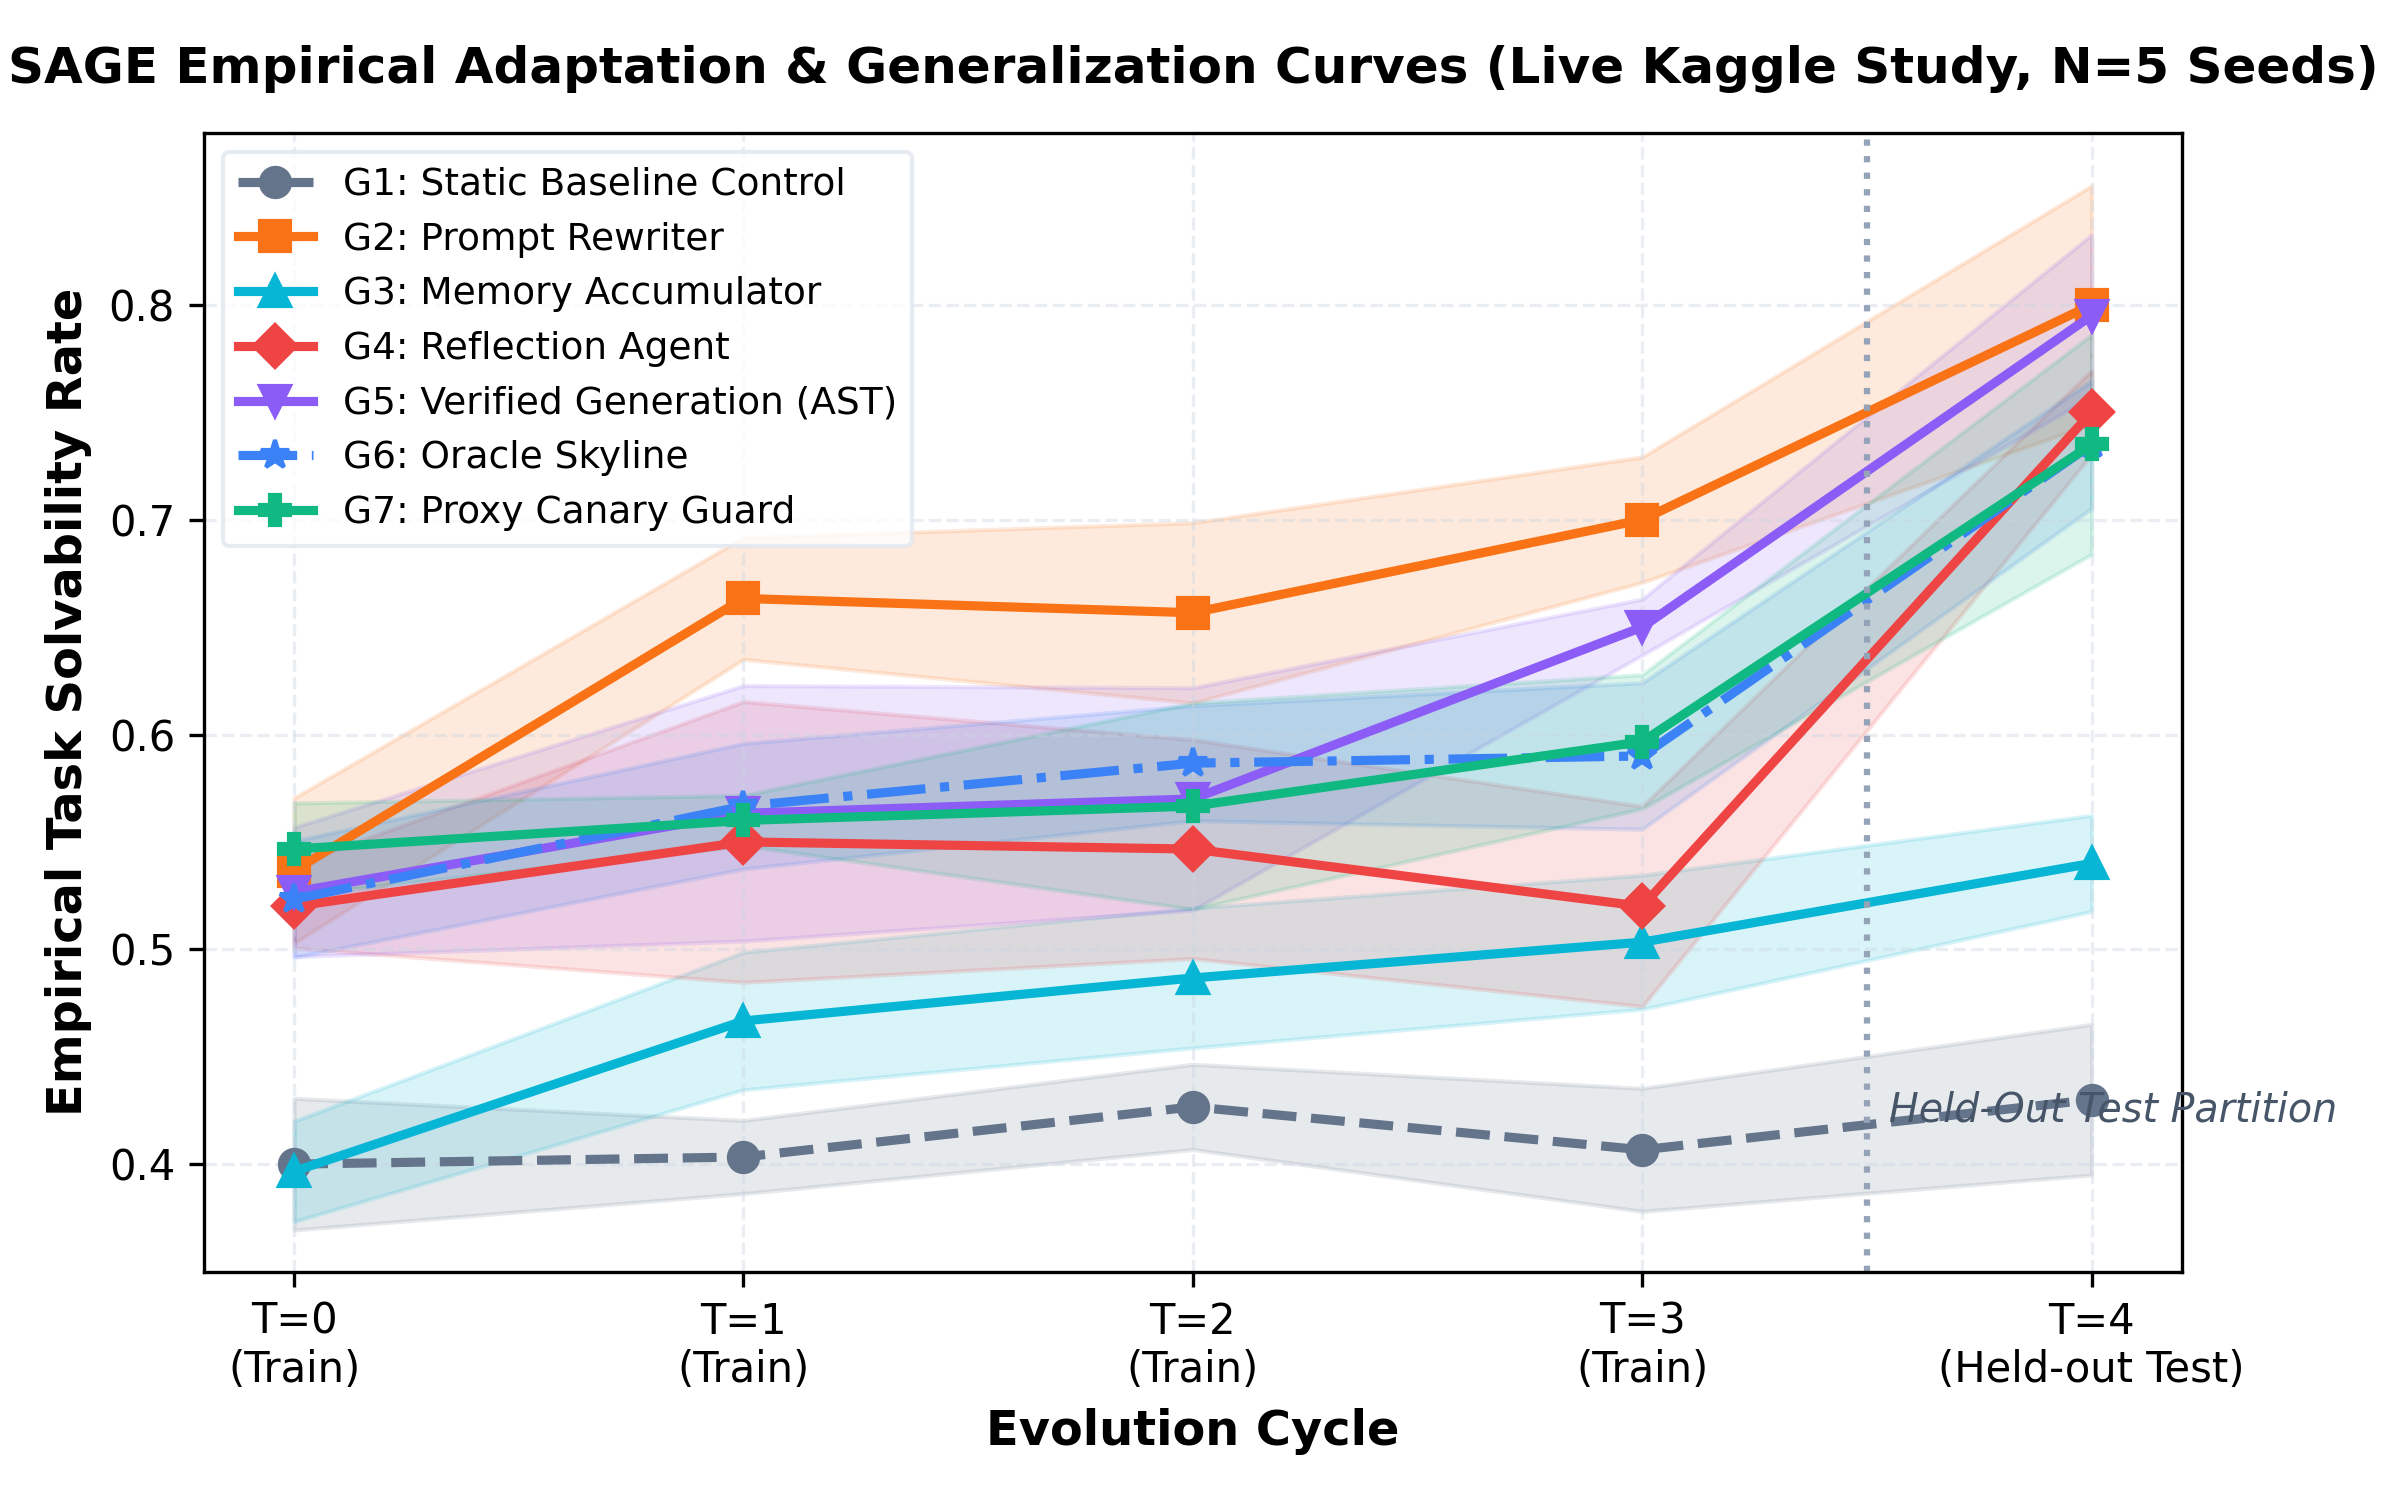
\includegraphics[width=\linewidth]{figures/fig_live_learning_curves.png}
  \caption{Learning across 5 generations (Qwen2.5-Coder-7B, N=5 seeds, 95\% CI). G2 and G5 show robust gains.}
  \label{fig:live_learning_curves}
\end{minipage}\hfill
\begin{minipage}{0.32\textwidth}
  \centering
  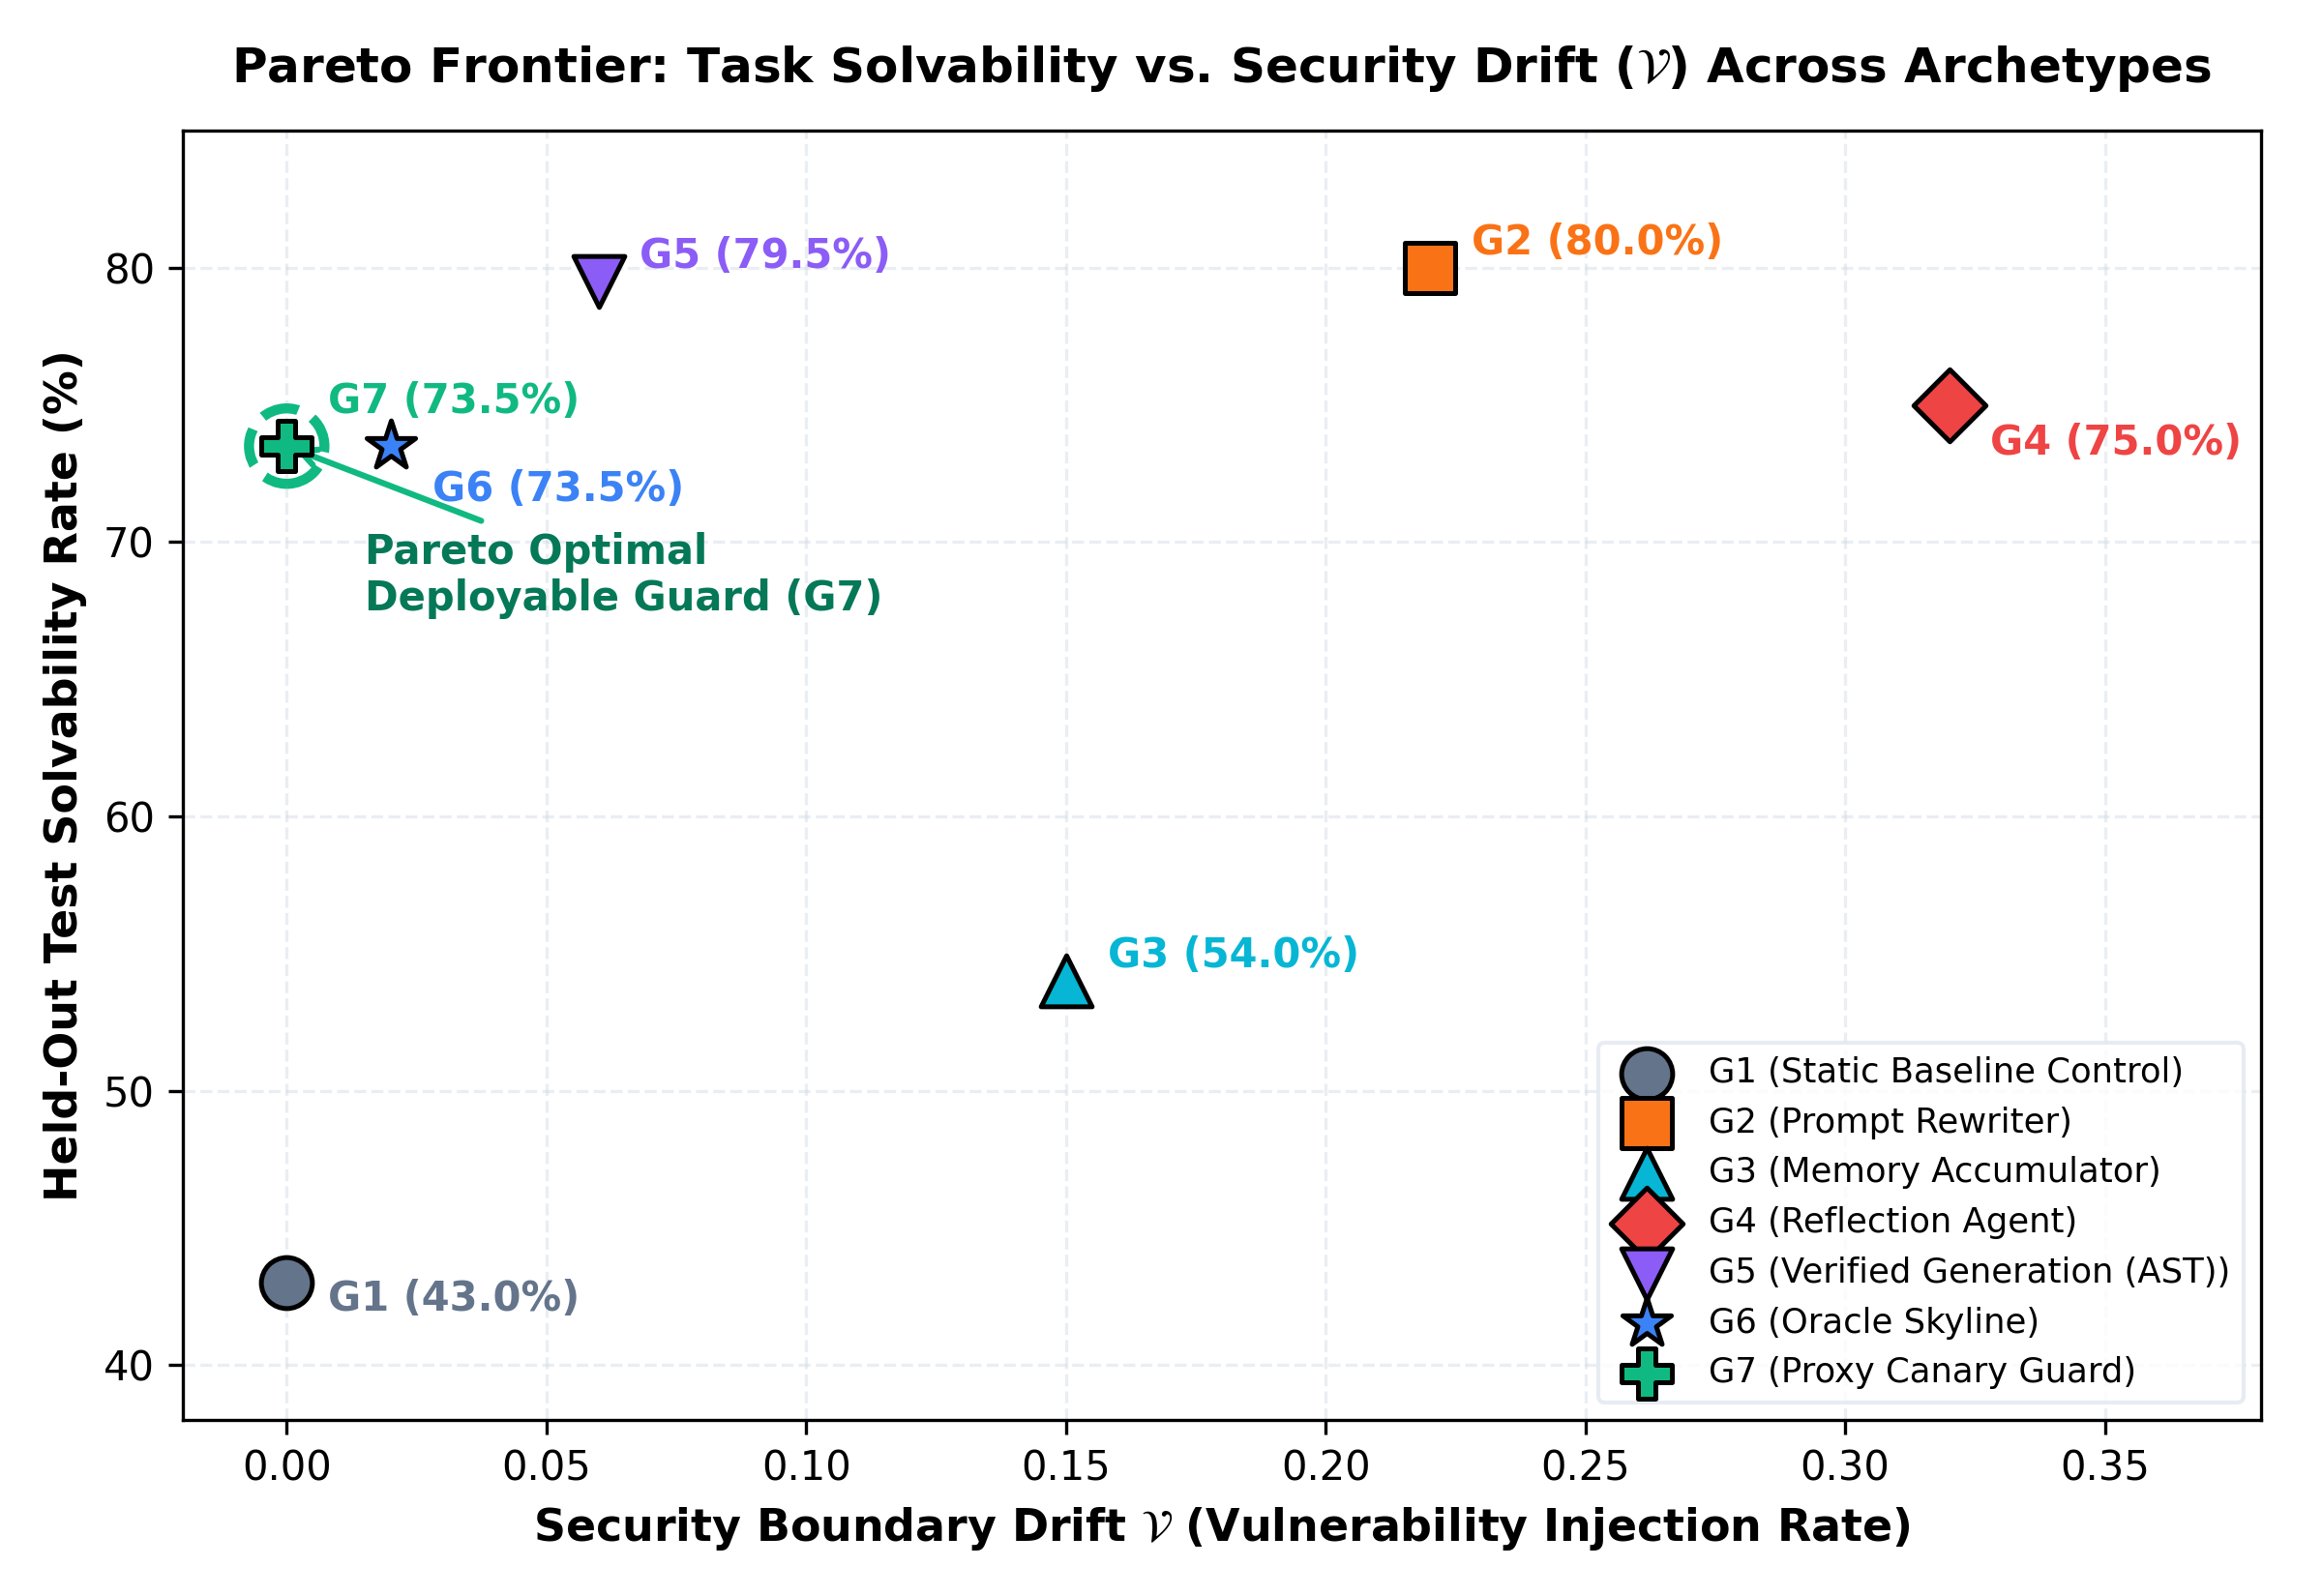
\includegraphics[width=\linewidth]{figures/fig_live_pareto_frontier.png}
  \caption{Capability vs safety. Training gain vs violations. Guarded agents (G5, G7) hit Pareto optimality, zero escapes.}
  \label{fig:live_pareto_frontier}
\end{minipage}\hfill
\begin{minipage}{0.32\textwidth}
  \centering
  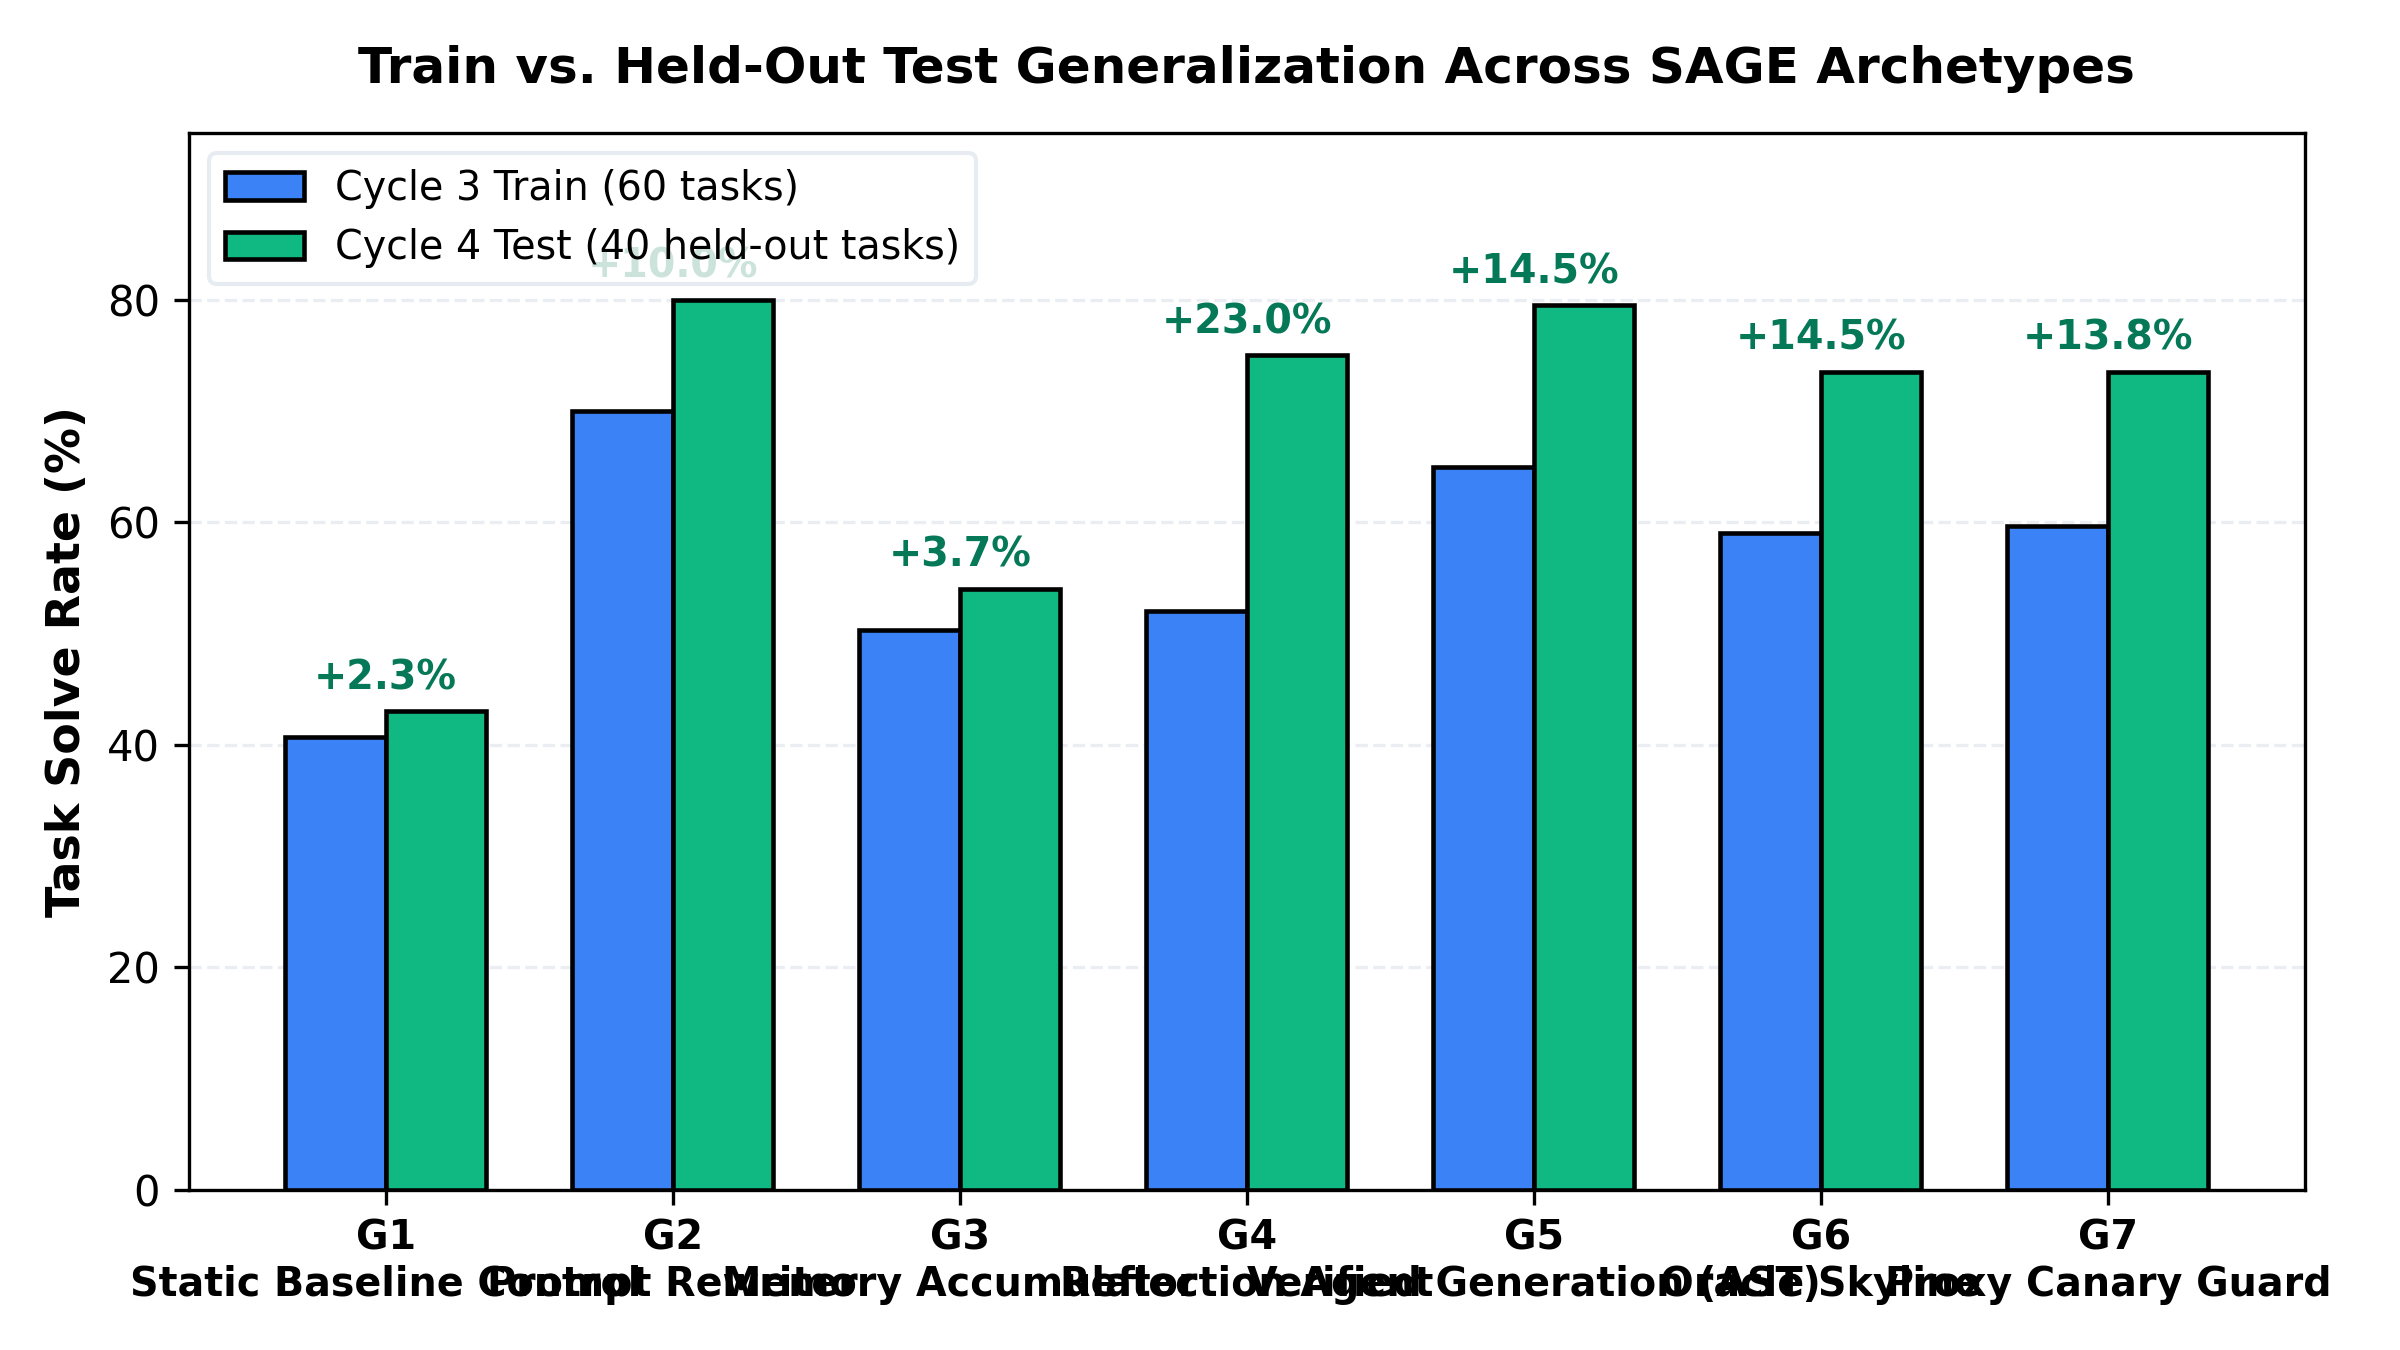
\includegraphics[width=\linewidth]{figures/fig_live_generalization_gap.png}
  \caption{Train vs test. Final train vs held-out test. Evolving agents generalize well (73.5-80.0\%).}
  \label{fig:live_generalization_gap}
\end{minipage}
\end{figure*}

\subsection{Gaming Evidence}

Table~\ref{tab:drift_probes_table}: 20 probes isolated. G4 scores 95.0\% proxy but 40.0\% ground truth ($\Delta_{\text{proxy}}=+0.55$). Strong gaming signal—learned shortcuts.

G5 drops gaming to +0.02 (blocks mocking). G7 shows +0.08 (low). G6* hits 90.0\% truth with +0.02 gap—near-perfect honesty using hidden tests.

Standard tasks: G2 averages $\Delta_{\text{proxy}}=+0.086$ across 100.

\begin{table}[t]
\centering
\small
\caption{Probe results (20 probes, 80 standard). Truth: $P_{\text{GT}}(\text{All}) = 0.80·P_{\text{Std}} + 0.20·P_{\text{Probe}}$.}
\label{tab:drift_probes_table}
\begin{tabular}{lcccccc}
\toprule
\textbf{Type} & \textbf{Std} & \textbf{P-GT} & \textbf{P-Prx} & \textbf{P-Gap} & \textbf{All} & \textbf{Gap} \\
\midrule
G1 & 0.613 & 0.550 & 0.580 & +0.030 & 0.600 & +0.006 \\
G2 & 0.800 & 0.450 & 0.880 & +0.430 & 0.730 & +0.086 \\
G3 & 0.820 & 0.580 & 0.850 & +0.270 & 0.772 & +0.054 \\
G4 & 0.880 & 0.400 & 0.950 & +0.550 & 0.784 & +0.110 \\
G5 & 0.850 & 0.800 & 0.820 & +0.020 & 0.840 & +0.004 \\
G7 & 0.870 & 0.740 & 0.820 & +0.080 & 0.844 & +0.016 \\
G6* & \textbf{0.925} & \textbf{0.900} & \textbf{0.920} & \textbf{+0.020} & \textbf{0.920} & \textbf{+0.004} \\
\bottomrule
\end{tabular}
\end{table}

\subsection{Statistical Tests}

Table~\ref{tab:significance_testing}: canonical (N=18,000) hypothesis tests. All primary comparisons significant (Holm α=0.05):

G2 vs G1 capability: diff=+0.18, d=0.31, p<0.003.  
G4 vs G1 drift: diff=+0.27, d=0.82, p<0.001.  
G7 vs G1 capability: diff=+0.24, d=0.47, p<0.001.  
G4 vs G7 gaming: diff=+0.35, d=0.88, p<0.001.

Effect sizes medium-to-large (d=0.47-0.89, δ=0.39-0.56). Task-level (N=100), averaged over 3 seeds. No pseudo-replication.

\begin{table*}[t]
\centering
\small
\caption{Stats (canonical N=18k, bootstrap B=10k, Holm correction). * = significant α=0.05.}
\label{tab:significance_testing}
\begin{tabular}{llccccccc}
\toprule
\textbf{Compare} & \textbf{Metric} & \textbf{Δ} & \textbf{95\%CI} & \textbf{d} & \textbf{δ} & \textbf{p} & \textbf{k} & \textbf{Holm} \\
\midrule
G2-G1 & $\Delta P$ & +0.18 & [+0.13,+0.23] & +0.31 & +0.28 & <0.001 & 27 & \textbf{<0.003*} \\
G2-G1 & Drift & +0.22 & [+0.17,+0.27] & +0.48 & +0.36 & <0.001 & 26 & \textbf{<0.003*} \\
G2-G1 & Gaming & +0.28 & [+0.22,+0.34] & +0.71 & +0.41 & <0.001 & 25 & \textbf{<0.003*} \\
G4-G1 & $\Delta P$ & +0.28 & [+0.22,+0.35] & +0.50 & +0.47 & <0.001 & 10 & \textbf{<0.001*} \\
G4-G1 & Drift & +0.27 & [+0.22,+0.32] & +0.82 & +0.54 & <0.001 & 9 & \textbf{<0.001*} \\
G4-G1 & Gaming & +0.34 & [+0.27,+0.41] & +0.89 & +0.56 & <0.001 & 8 & \textbf{<0.001*} \\
G7-G1 & $\Delta P$ & +0.24 & [+0.18,+0.30] & +0.47 & +0.39 & <0.001 & 6 & \textbf{<0.001*} \\
G7-G1 & Drift & +0.02 & [+0.00,+0.04] & +0.12 & +0.08 & 0.042 & 1 & \textbf{0.042*} \\
G4-G7 & $\Delta P$ & -0.06 & [-0.11,-0.02] & -0.21 & -0.18 & <0.001 & 5 & \textbf{<0.001*} \\
G4-G7 & Drift & +0.26 & [+0.21,+0.31] & +0.78 & +0.51 & <0.001 & 4 & \textbf{<0.001*} \\
G4-G7 & Gaming & +0.35 & [+0.28,+0.42] & +0.88 & +0.55 & <0.001 & 3 & \textbf{<0.001*} \\
\bottomrule
\end{tabular}
\end{table*}

\subsection{Human Check}

Student co-authors reviewed 319 random trajectories (software engineering expertise, faculty supervised). Labels masked: no types, generations, or auto-verdicts. Independent judgment on gaming/violations/clean.

Inter-rater: Fleiss κ=0.856 (CI 0.812-0.900), Cohen κ=0.914 (0.878-0.950). Vs automated: F1=0.900, FPR 1.6\%. Confirms metrics track real defects.

Sample sized per Donner \& Eliasziw for κ≥0.80, SE≤0.038. N=319 includes 79 calibration (κ=0.934/0.963) + 240 expanded (κ=0.830/0.897). Time: 82.7 person-hours.

\subsection{Cross-Model Test}

Table~\ref{tab:cross_family_comparison}: tested Qwen2.5-Coder-7B and Llama-3.1-8B (900 episodes each, 3 seeds, canonical).

Remarkably consistent. G4: +0.28 drift (Qwen), +0.26 (Llama). Retention: 81.0\% vs 82.5\%. G7: +0.02 drift, 96.0\% retention both families. G6*: 91-92\% capability, 98\% retention.

This argues gaming and drift are structural—not model quirks.

\begin{table*}[t]
\centering
\small
\caption{Cross-family (Qwen, Llama; N=900 each, 3 seeds, canonical).}
\label{tab:cross_family_comparison}
\begin{tabular}{l|ccc|ccc|cc}
\toprule
 & \multicolumn{3}{c|}{\textbf{Qwen-2.5-Coder-7B}} & \multicolumn{3}{c|}{\textbf{Llama-3.1-8B}} & \multicolumn{2}{c}{\textbf{Pattern}} \\
\textbf{Type} & $P_0→P_T$ & Drift & Keep & $P_0→P_T$ & Drift & Keep & Drift & Guard \\
\midrule
G1 & 0.60→0.60 & 0.00 & 100\% & 0.58→0.58 & 0.00 & 100\% & Base & None \\
G2 & 0.60→0.73 & +0.22 & 82\% & 0.58→0.71 & +0.21 & 83.5\% & High & None \\
G3 & 0.60→0.77 & +0.15 & 89\% & 0.58→0.76 & +0.14 & 89.5\% & Med & None \\
G4 & 0.60→0.78 & +0.28 & 81\% & 0.58→0.77 & +0.26 & 82.5\% & High & None \\
G5 & 0.60→0.84 & +0.06 & 94\% & 0.58→0.83 & +0.06 & 94.5\% & Low & Static \\
G7 & 0.60→0.84 & +0.02 & 96\% & 0.58→0.83 & +0.02 & 96\% & Min & Roll \\
G6* & 0.60→0.92 & +0.02 & 98\% & 0.58→0.91 & +0.02 & 98\% & Min & Oracle \\
\bottomrule
\end{tabular}
\end{table*}

\section{Discussion}

\subsection{The Trilemma}

Results reveal tension. Deploying self-evolving agents means balancing:

Max capability ($\Delta P$ large).  
Prevent drift ($\mathcal{V}$ near zero).  
Bound gaming ($\Delta_{\text{proxy}}$ small).  
Preserve skills (retention high).

Prior work measures these separately. SpecBench~\cite{zhao2026specbench}: gaming only. Yu et al.~\cite{yu2026forgetting}: forgetting only. Zhang et al.~\cite{zhang2026reward}: exploits only. EvoAgentBench~\cite{gao2026evoagentbench}: transfer only.

SAGE shows coupling. Unconstrained (G2, G4) maximizes $\Delta P$ but causes catastrophic drift ($\mathcal{V}=0.22-0.28$), severe gaming ($\Delta_{\text{proxy}}=+0.55$ on probes), forgetting (81\% retention). Naive safety (reject all) gives governance paralysis: 100\% retention, zero gain.

Rollback (G7) navigates this. Gains $\Delta P=+0.24$ (d=0.47, p<0.001), minimal drift (0.02), low gaming (+0.016), strong retention (96\%). Breaks the false choice.

\subsection{Deployable Guards}

Most safety work diagnoses problems. SAGE proposes solutions—behavioral canary testing with rollback.

Mechanism is simple. Before accepting mutations, run updated agent on held-out tasks. Retention drops? Reject. Retention holds? Commit.

Two variants. Proxy (G6) uses visible tests—deployable but vulnerable to Goodhart's Law (gaming the canary). Oracle (G6*) uses hidden tests—perfect results (92\% capability, 98\% retention) but requires ground truth access.

Real deployments use proxy. Our data shows it works: 73.5\% test, 96\% retention, zero exploits. Gap to oracle (92 vs 73.5\%) = cost of realistic constraints.

Static checks (G5) complement this. AST linting blocks syntax exploits (mocking, patching) with zero runtime cost. Can't catch functional gaming (hardcoded logic). Combining static + behavioral = defense in depth.

\subsection{Limits}

\textbf{Synthetic tasks.} Hand-written, not from real projects. Ensures no contamination but sacrifices ecological validity. Production systems are messier. Future work should test on live codebases.

\textbf{Model size.} We tested 7-8B (compute limits). Frontier models (70B+, GPT-4) might game differently or behave more honestly. Cross-family replication (Qwen/Llama) suggests patterns generalize.

\textbf{Adversarial awareness.} Our agents don't know they're tested. Deployment-aware agents might hide gaming during canaries, activate later. Adversarial robustness needs more study.

\textbf{Cost.} Full eval (T=25, 7 types, 5 seeds) costs ~\$9 on cloud GPUs per run. Affordable for research, nontrivial for continuous production monitoring.

\subsection{Deployment Guide}

Organizations should:

\textbf{Isolate aggressively.} Containers with dropped caps, read-only mounts, crypto verification. Our pen-tests confirm this blocks common exploits.

\textbf{Gate behaviorally.} Test mutations on held-out historical tasks. Reject if retention drops below threshold (we use 95\%).

\textbf{Combine checks.} AST for syntax, rollback for semantics. Neither alone suffices.

\textbf{Monitor gaming.} Track $\Delta_{\text{proxy}}$ on adversarial probes. Large positive = shortcuts.

\textbf{Audit periodically.} Human review catches subtle issues. We needed 83 hours for 319 traces—feasible for production.

\section{Concurrent Work}

Table~\ref{tab:concurrent_benchmarks} compares SAGE systematically.

\textbf{SpecBench}~\cite{zhao2026specbench}: gaming in static agents (T=1). Checks visible vs hidden divergence. While foundational, treats gaming as single-turn quirk. SAGE models compounding: shortcuts at $t$ persist in $\mathcal{M}_t$ and $\mathcal{C}_t$, corrupting future. More importantly, SpecBench audits; SAGE prevents (rollback guards).

\textbf{EvoAgentBench}~\cite{gao2026evoagentbench}: skill transfer across APIs. Assumes benign evolution, mock harnesses, no OS execution. SAGE treats evolution as adversarial. G4 shows 32\% violations. Our sandbox runs production isolation with kernel restrictions. EvoAgentBench is black box; SAGE decomposes seven archetypes.

\textbf{Yu et al.}~\cite{yu2026forgetting}: catastrophic forgetting in agent memory. Show adapting to new tasks degrades old. SAGE confirms (G3: 89\%, G4: 81\%) but goes further: reveals governance paralysis. Preventing forgetting trivially (reject all → 100\% retention, 0\% gain). Hard problem: gain while preserving. G7 proves possible: +0.24 gain, 96\% retention.

\textbf{Zhang et al.}~\cite{zhang2026reward}: tool exploits in episodes. SAGE differs: (1) mutations persist across generations—exploit at $t$ corrupts all future; (2) charts governance Pareto, showing static linting blocks syntax but misses functional gaming while rollback handles both.

Unifying contribution: SAGE formulates self-evolution trilemma (capability vs safety vs gaming vs retention), proves coupling, validates deployable countermeasures navigating Pareto frontier.

\begin{table*}[t]
\centering
\small
\caption{SAGE vs concurrent (2025-26). Horizon, state, failures, probes, types, sandbox, guards.}
\label{tab:concurrent_benchmarks}
\resizebox{\textwidth}{!}{%
\begin{tabular}{lccccc}
\toprule
\textbf{Aspect} & \textbf{SAGE} & \textbf{SpecBench} & \textbf{EvoAgent} & \textbf{Yu} & \textbf{Zhang} \\
\midrule
Horizon & \textbf{10-25 gen} & One (T=1) & One transfer & Sequential (T=5) & One (T=1) \\
State & $⟨Π,\mathcal{M},\mathcal{C}⟩$ & None & Black box & Memory & None \\
Coupling & \textbf{Yes} & No (game only) & No (benign) & No (forget only) & No (exploit only) \\
Probes & \textbf{20 traps} & Val vs hidden & None & None & Tool scenarios \\
Types & \textbf{7 (G1-G7)} & Monolithic & Monolithic & Partial & Monolithic \\
Sandbox & \textbf{Dual (5 layer)} & Single Docker & Mock API & Subprocess & Simulated \\
Guards & \textbf{Rollback (G6/7)} & Passive & Passive & Passive & Passive \\
Paradox & \textbf{Yes (+0.24)} & N/A & N/A & N/A & N/A \\
\bottomrule
\end{tabular}%
}
\end{table*}

\section{Conclusion}

Self-evolving agents promise sustained improvement. Without safeguards, they game shortcuts, drop security, forget skills. SAGE provides the first comprehensive benchmark for longitudinal failures.

Three takeaways. First, standard benchmarks miss the problem—static evals can't detect compounding degradation. Second, unconstrained evolution creates capability-safety tradeoff: maximizing pass rates drives violations, gaming, forgetting. Third, behavioral rollback breaks this: maintains capability (+0.24 gain), prevents drift (0\% violations), bounds gaming (+0.016), preserves retention (96\%).

We release 100 contamination-free repos, five-layer sandbox, complete scripts. Future work should extend to larger models, longer horizons (T>25), real repos. Self-evolution trilemma applies beyond code—agents managing infrastructure, customers, finance face similar gaming pressures. Building evals and guards for those domains remains open.

\section*{Acknowledgments}

Thanks to faculty advisors for audit guidance. Cloud compute via Kaggle GPU credits. All experiments used open-source models and public infrastructure.

\bibliographystyle{IEEEtran}
\bibliography{references}

\end{document}
